\chapter{Testing \& Evaluation} \label{cha:testing}
\section{Using the System}
To test Aims and Objectives 1 \& 2, \todo{finish this section}

for All tests in this section a Raspberry Pi 4b was used to host client code, running Raspberry Pi OS Lite (with no desktop environment), which was released on December 11th 2023. The server and frontend were hosted on a Laptop with an Intel i5-12450H processor, running Fedora 39 Linux. The Raspberry Pi's hostname (visible in screenshots) is "nikpi".
\subsection{Controlling one connected device} \label{cha:testing:onedevice}
Perhaps the most obvious and basic test is to create a device, using the Rust client library, have it run on a device and to connect with that device to a running server. 

\subsubsection{Testing Setup}
A simple client was created, with two capabilities "Turn On" and "Turn Off". The callback functions attached to these capabilities would simply log to the standard output the name of the capability they are attached to. The Raspberry Pi is connected to the same Wi-Fi network as the server. The port 2302 has opened on the laptop's firewall to ensure the Raspberry Pi can make requests to the gRPC server. The Raspberry Pi is being controlled through a secure shell connection (SSH) (visible on the left side of screenshots). View figure~\ref{fig:example_config_raspi} for the exact configuration of the client.
\begin{figure}[h]
\caption{Client's configuration file}
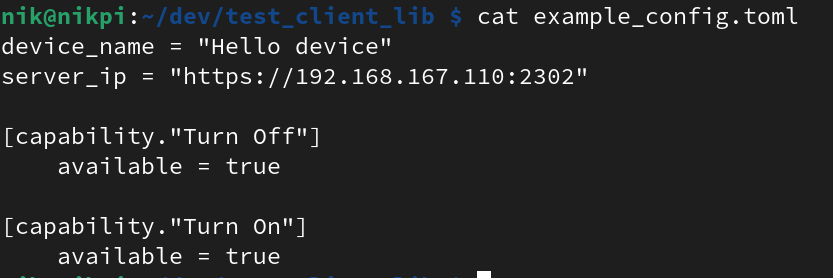
\includegraphics[width=\textwidth]{example_config_raspi}
\label{fig:example_config_raspi}
\end{figure}

\subsubsection{Testing}
Figure~\ref{fig:establish_connection_raspi} shows the successful connection and certificate exchange between the client on nikpi and the server. Note that the server ip that the client is connecting to is set within the client's configuration file (view figure~\ref{fig:example_config_raspi}). In this case the server (on the right side of figure~\ref{fig:establish_connection_raspi}) is being started with the "json-frontend" flag, as discussed within subsection~\ref{sec:chapimpl:frontend:json}, this flag is required to use the web-based frontend.
\begin{figure}[h]
\caption{Establishing a connection }
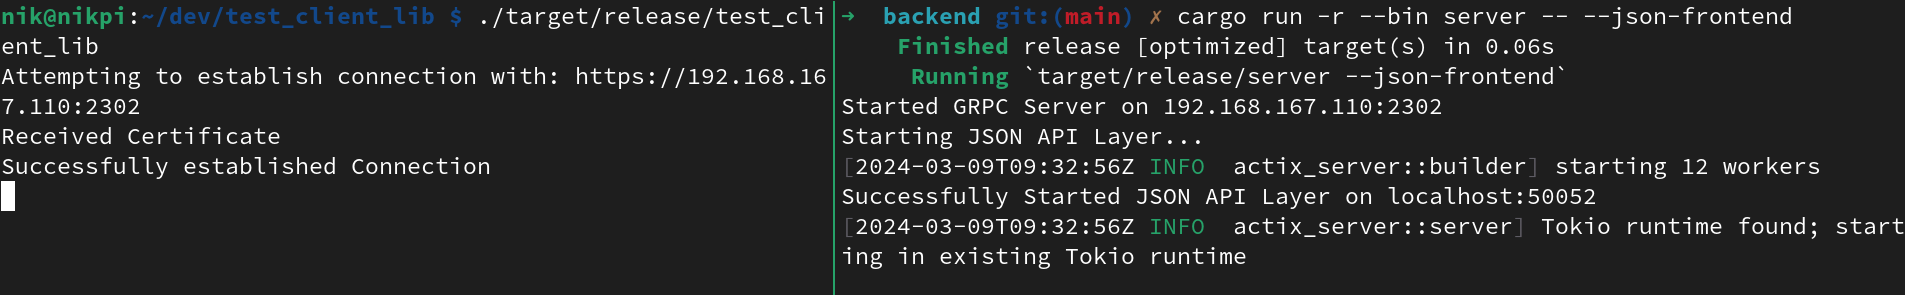
\includegraphics[width=\textwidth]{establish_connection_raspi}
\label{fig:establish_connection_raspi}
\end{figure}

The next important test is viewing the web frontend, to see that the device is correctly displayed on the frontend, with the appropriate capabilities. This can be seen in figure~\ref{fig:web_frontend_one_connected_device}, where the device, named "Hello device" (view configuration file) can be seen with it's two capabilities "Turn Off" and "Turn On". The web-frontend is being hosted by a Vite server, through using the command "npm run dev", on localhost port 5173. The frontend is being rendered by the Chromium web browser.
\begin{figure}[h]
\caption{Web Frontend with the connected device}
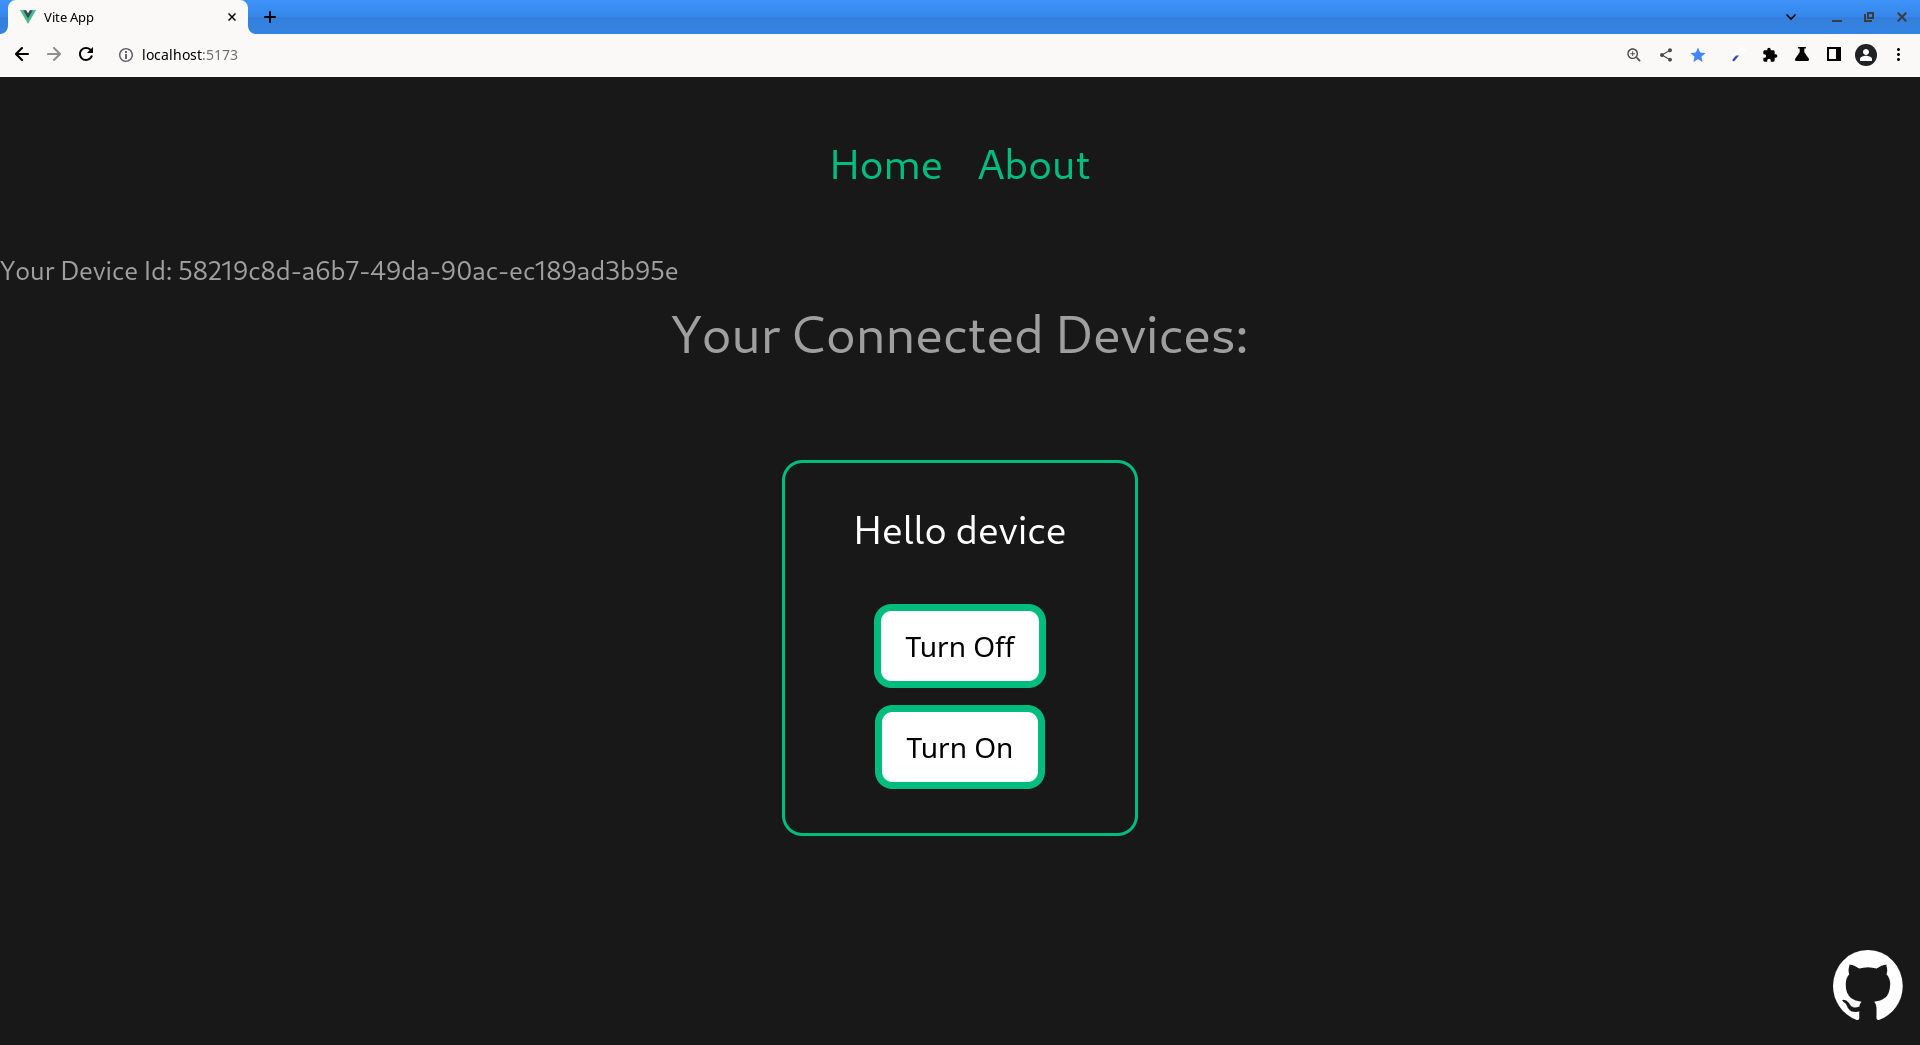
\includegraphics[width=\textwidth]{testing_web_frontend_one_device}
\label{fig:web_frontend_one_connected_device}
\end{figure}

The final test for this subsection is to attempt to trigger the two listed capabilities, by clicking the buttons. This should send a JSON packet to the JSON proxy server, which is then forwarded to the gRPC server. Once this request has been processed, the server will add it to the list of updates for the specified client. The client will then eventually poll the server and receive the update. It will then call the callback function associated with that capability. For this specific test both buttons will be clicked, starting with the "Turn Off" button, then the "Turn On Button". As shown in figure~\ref{fig:triggering_capability} this works as expected and the associated callback functions are called.
\begin{figure}[h]
\caption{Triggering capabilities}
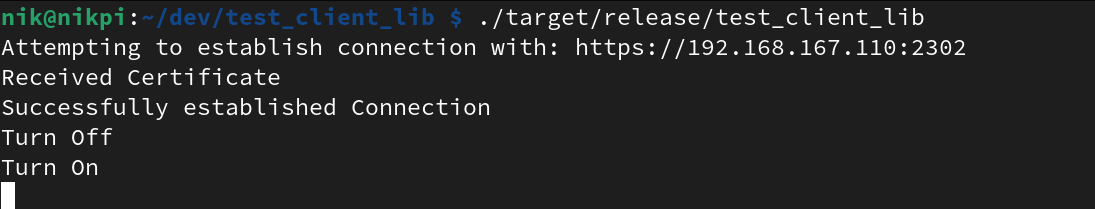
\includegraphics[width=\textwidth]{toggle_turn_on_off}
\label{fig:triggering_capability}
\end{figure}

You can view the complete code for the client used in this example in the appendix in appendix section~\ref{chap:A2:onedeviceclientlib}. Due to the simplicity of setting up a client using the NOSHP-Client library, its only 47 lines long.

\subsection{Controlling multiple connected devices}
This section will be a continuation of the last section, except that multiple devices will now be run, instead of just one. One device will still be run off the Raspberry Pi, the other devices will be run locally, on the server. They will however still be connecting to the public IP Address, not the loop-back address. Running them on the same device as the server has potential performance implications, however it is not relevant to this section, as we are simply attempting to test the functionality of the system.

\subsubsection{Testing}
One slight modification has been made to the code in appendix section~\ref{chap:A2:onedeviceclientlib}, a print statement has been added to the main function, which prints the device name to standard output. This aids in clarity for which device is which in the screenshots. Additionally, configurations have slightly changed, with each device having uniquely named capabilities and device names, to demonstrate the frontend's ability to show different devices. The IP address they are connecting to will stay the same (the server's IP printed at startup).

\begin{figure}[h]
\caption{Establishing Connection with four devices}
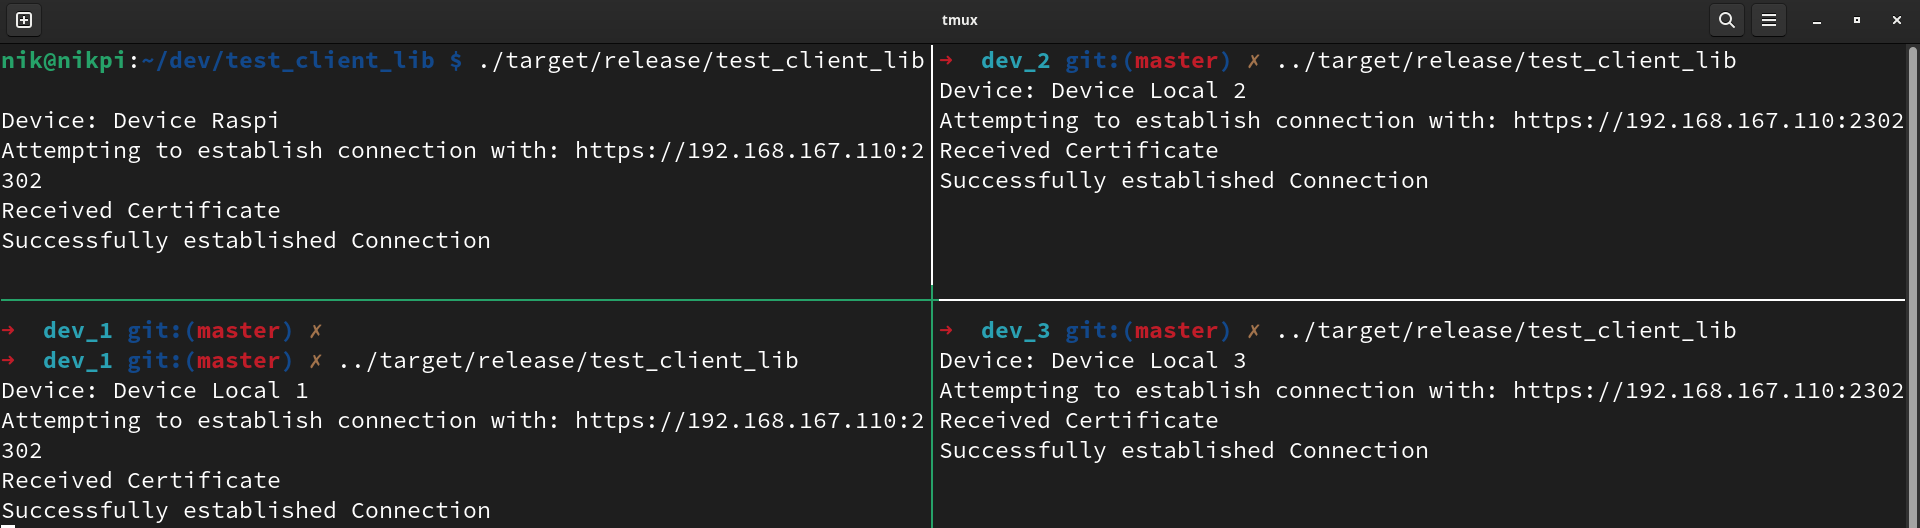
\includegraphics[width=\textwidth]{testing_four_devices_connection.png}
\label{fig:four_connected_device_connection}
\end{figure}
As seen in figure~\ref{fig:four_connected_device_connection}, connecting four devices the server is no problem. All four connect, receive their certificate and print that they have successfully established their connection. The next test is to see that all are displayed properly on the frontend, with the correct device names and capability names.


\begin{figure}[h]
\caption{Web-frontend with four devices}
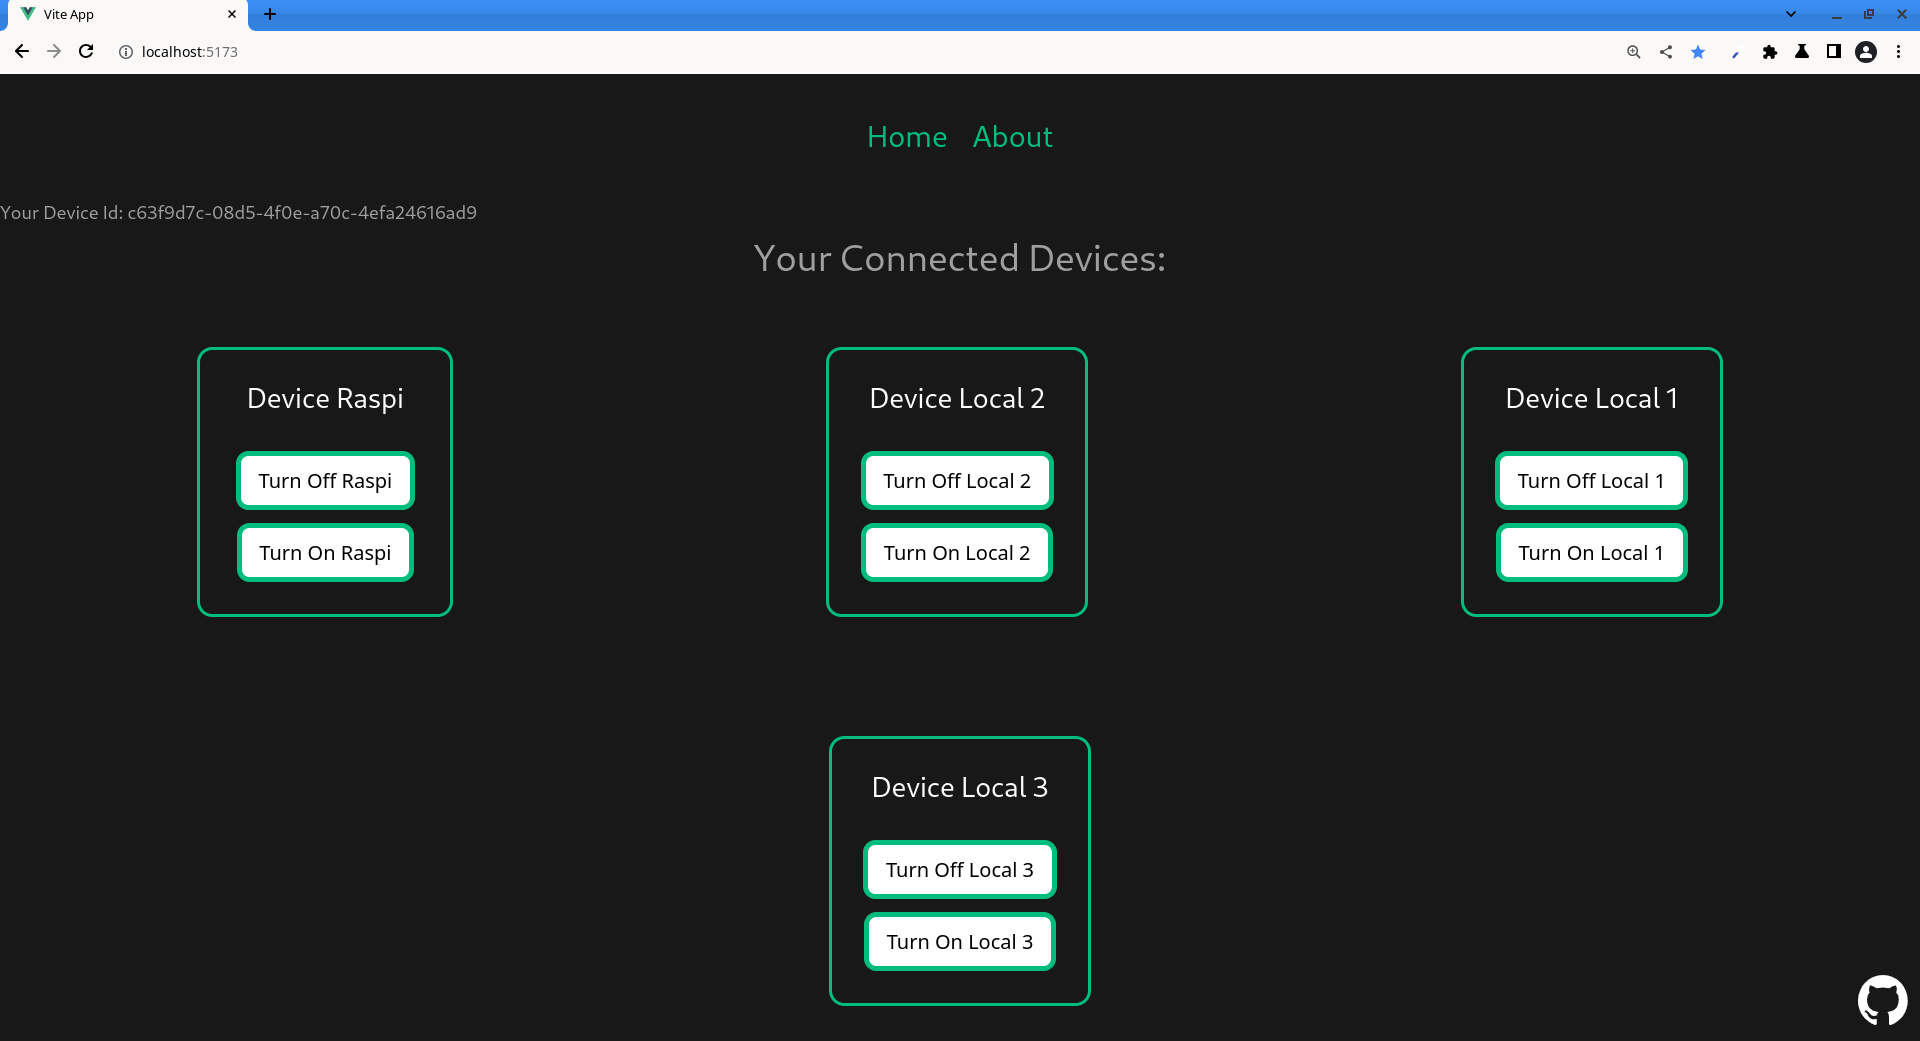
\includegraphics[width=\textwidth]{testing_four_devices_frontend.png}
\label{fig:four_connected_device_frontend}
\end{figure}
Figure~\ref{fig:four_connected_device_frontend} shows all four devices, with their correct names and capabilities displayed on the web frontend. Note that nothing has been changed about the frontend during this time, this has all been dynamically changed due to changing connected devices. Finally, we must test controlling each of the four devices. This was done by clicking every button seen on screen, from left to right and top to bottom order. The results from this can be seen in figure~\ref{fig:four_connected_device_toggle}.

\begin{figure}[h]
\caption{Triggering capabilities with four devices}
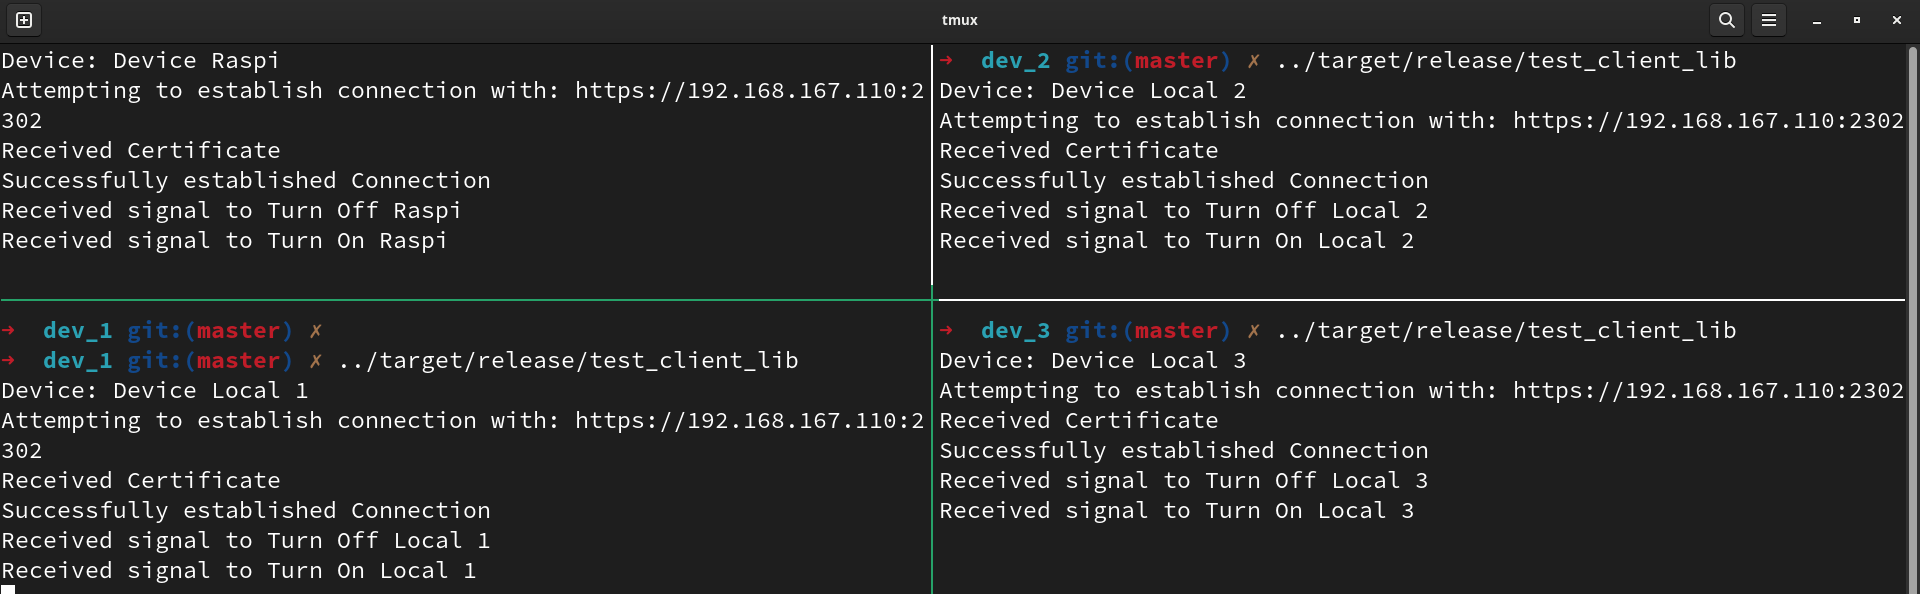
\includegraphics[width=\textwidth]{testing_four_devices_toggle.png}
\label{fig:four_connected_device_toggle}
\end{figure}
All four devices trigger their capabilities correctly. That being said, a potential issue was uncovered during this experiment. Due to latency between server and device (specifically the Raspberry Pi which was connected through Wi-Fi), packet signatures can expire before they reach the device. This can lead to lost information, as the server has already removed the update. While a somewhat rare problem, it could happen frequently on a faulty connection. An easy fix was to increase the amount of time it takes for a signature to expire, however a proper fix would for the client to send a response message, when the update has been received. The server would only delete updates when this message is received. 




\subsection{Sending incorrect signatures}
\section{Performance Testing}
\section{Issues found during testing}
- Currently if signature expires, then information is lost as it already has been deleted from the server.
